

\documentclass[pdf]{beamer}
\usepackage{graphicx}
\usepackage{pgf}
\usepackage{tikz}
\usetikzlibrary{arrows,shapes}
\usepackage{verbatim}
\usetheme{Boadilla}
\setbeamertemplate{navigation symbols}{}

\title[Finding efficient HCRs]{
Finding efficient harvest control rules for data limited management
	}
\subtitle{
	}
\author[CE \& FS]{
	Charles T T Edwards\textsuperscript{1} and Finlay Scott\textsuperscript{2}
	}
\institute[ICL and CEFAS]{
	\textsuperscript{1,2}Imperial College London, UK\\\textsuperscript{2}CEFAS, UK
	}
\date[WFC, May 2012]{World Fisheries Congress\\Edinburgh, May 2012}

\begin{document}



\frame{\titlepage}

\section{Introduction}
\begin{frame}
\frametitle{Introduction}
\structure{Objective:} to find control rules that perform well in data poor situations.
\begin{itemize}
\item How do we measure performance?
\item What do we mean by data poor?
\end{itemize}
\vspace{20pt}
\structure{Overview of study:}
\begin{itemize}
\item Introduce a measure of \alert{control rule performance}
\item Define control rules
\item Compare performance under different data scenarios
\item Quantify \alert{data uncertainty}
\item Compare performance relative to data uncertainty
\end{itemize}
\end{frame}

\section{Efficiency}
\begin{frame}
\frametitle{Efficiency}
\framesubtitle{How do we measure performance?}
Statistical efficiency measures the deviation of an estimated value $\hat{\theta}$ from the true value $\theta$:
\begin{equation}
e(f) = \frac{1/I(\theta)}{E[(\theta - \hat{\theta})^2]} \nonumber
\end{equation}
\vspace{20pt}\\
From this definition we obtain our measure of performance.
\begin{block}{}
\textcolor{blue}{Performance statistic:}
\vspace{5pt}
\begin{equation}
e(HCR) \propto \frac{1}{E[(C - \hat{C})^2]} \nonumber
\end{equation}
\vspace{5pt}
\end{block}
\end{frame}

\section{Harvest control rules}
\begin{frame}
\frametitle{Harvest control rules}
\framesubtitle{How do we calculate $C$ and $\hat{C}$?}
\begin{block}{}
\textcolor{blue}{Harvest control rule:}
\vspace{5pt}
\begin{equation}
C_{y+1} = \frac{I_{y+1}C^{TAR}}{I^{TAR}}\nonumber
\end{equation}
\vspace{5pt}
\end{block}
\vspace{20pt}
Tested four methods of predicting $\hat{I}_{y+1}\longrightarrow \hat{C}_{y+1}$:
\begin{itemize}
\item Moving average
\item Linear regression
\item Smoothed index
\item Model-based (Stock reduction analysis)
\end{itemize}
\end{frame}

\section{Data scenarios}
\begin{frame}
\frametitle{Data scenarios}
\framesubtitle{Information input for the control rule}
\begin{figure}
\includegraphics[width=0.6\textwidth]{../dat/obserror.pdf}
\end{figure}
\structure{Experimental design:} by changing the \alert{years of data} available to the control rule ($n$) and the \alert{observation error} ($\sigma$) we can modify the data uncertainty.
\end{frame}

\section{Simulation results}
\begin{frame}
\frametitle{Simulation results}
\framesubtitle{Illustrative results}
\begin{figure}
\includegraphics[width=0.9\textwidth]{../res/uncertainty_index.pdf}
\end{figure}
\end{frame}

\begin{frame}
\frametitle{Simulation results}
\only<1>{
\framesubtitle{Moving average control rule}
\begin{figure}
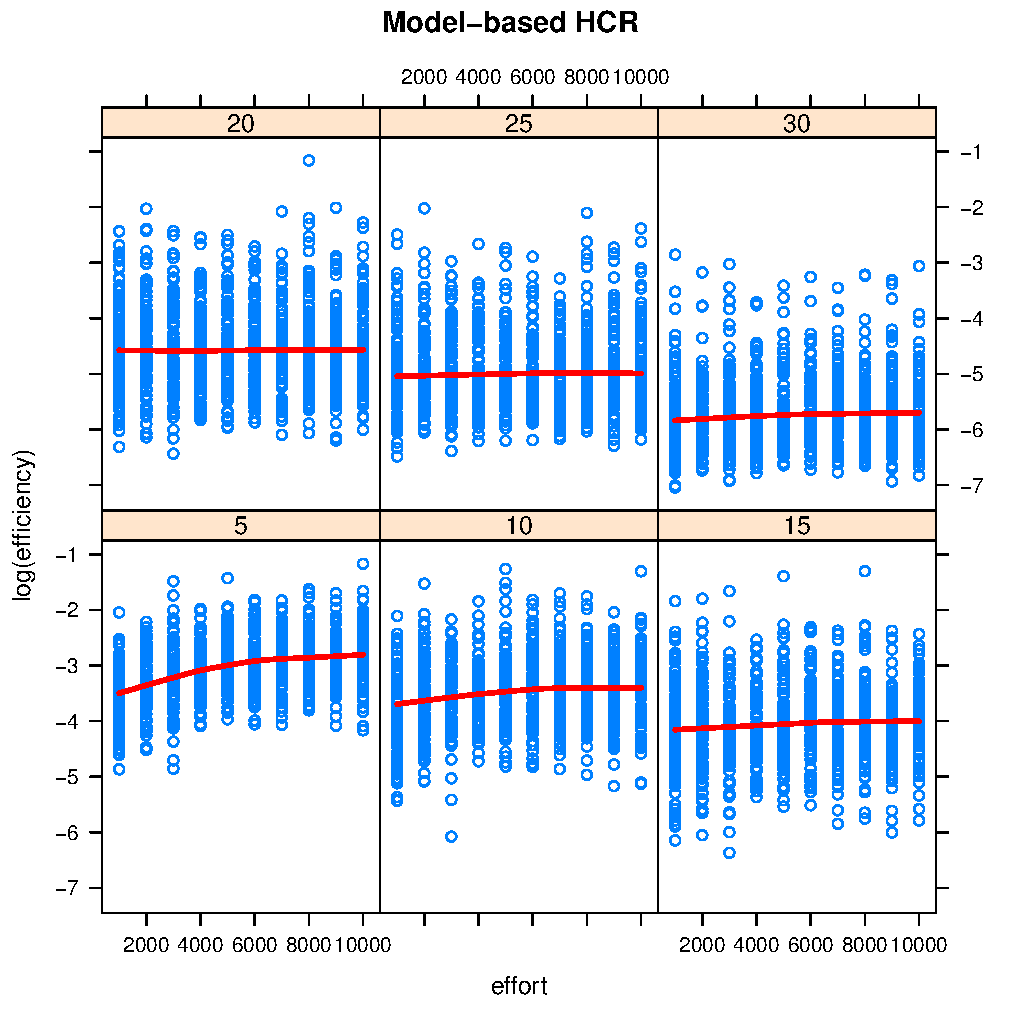
\includegraphics[width=1\textwidth]{../res/hcr_mav_plot2.pdf}
\end{figure}
}
\only<2>{
\framesubtitle{Regression-based control rule}
\begin{figure}
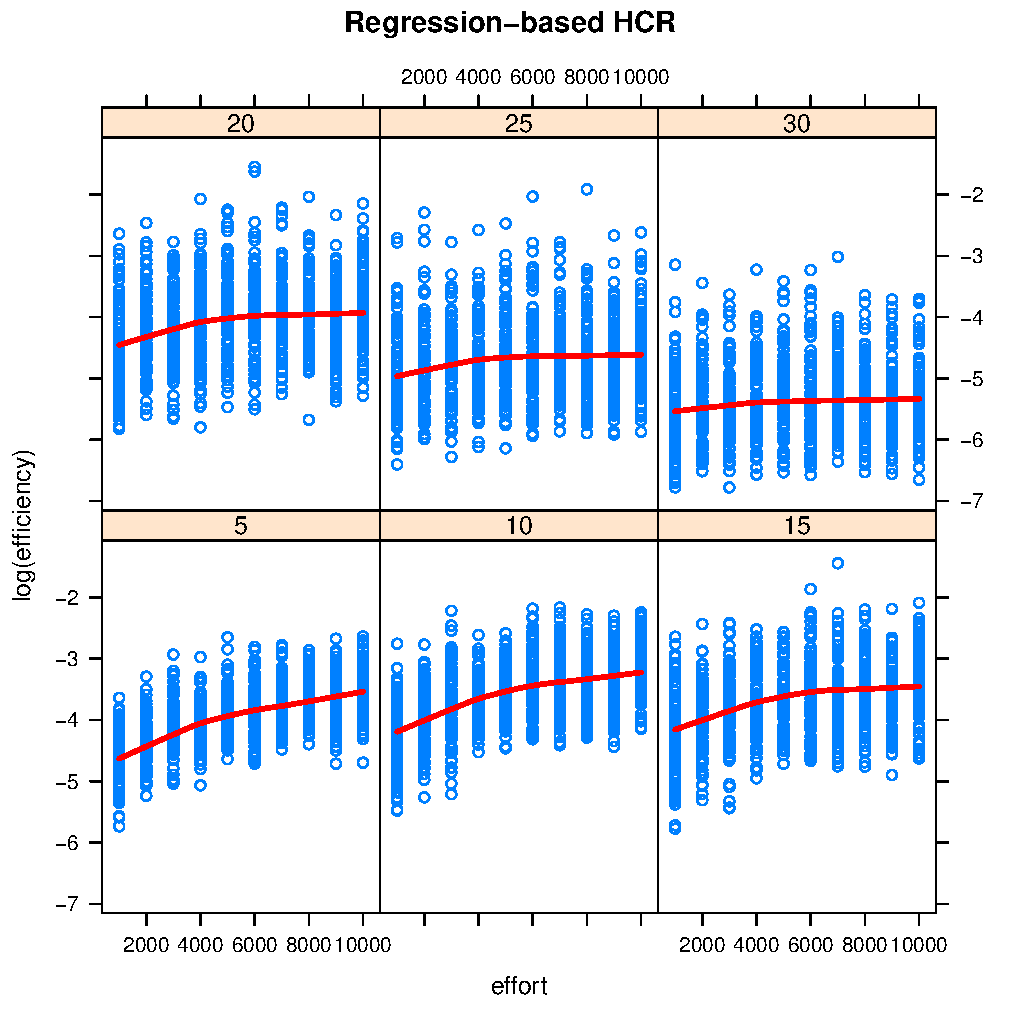
\includegraphics[width=1\textwidth]{../res/hcr_reg_plot2.pdf}
\end{figure}
}
\only<3>{
\framesubtitle{Smoothed index control rule}
\begin{figure}
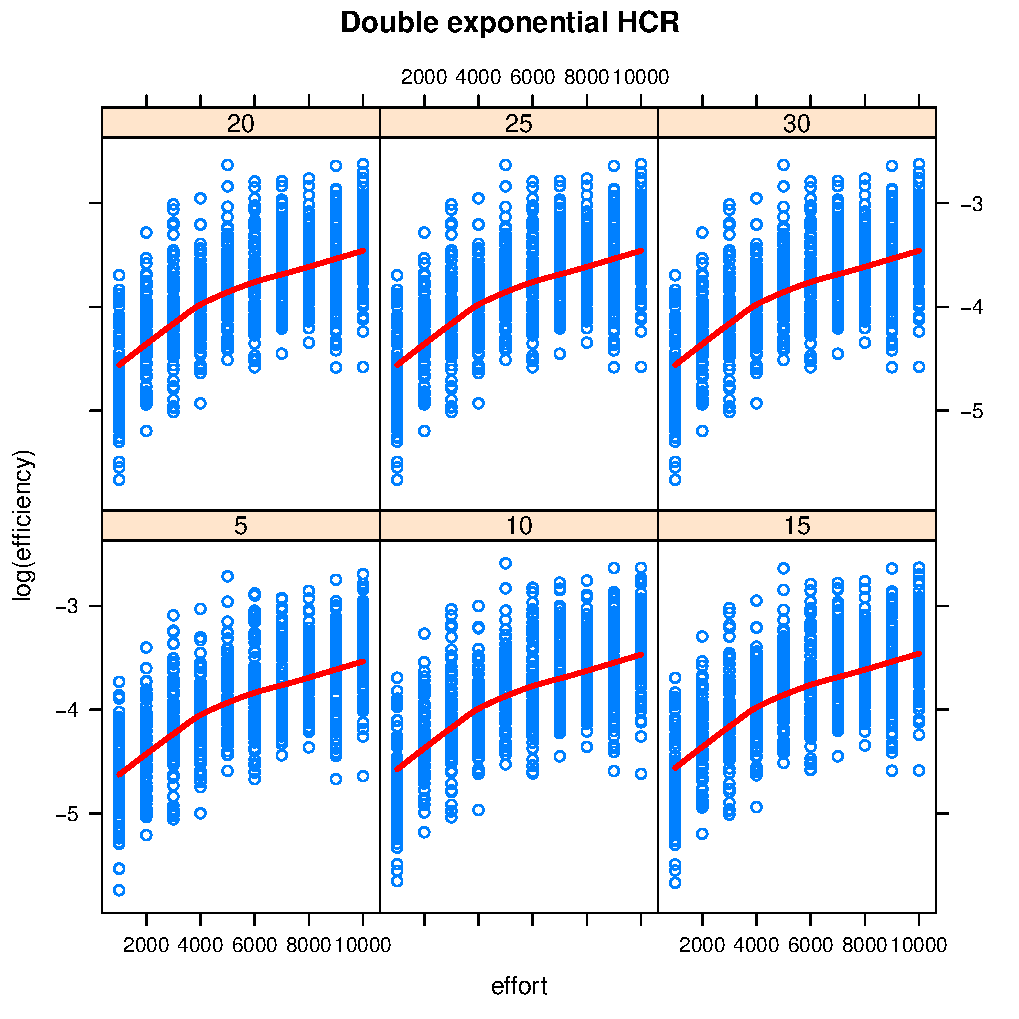
\includegraphics[width=1\textwidth]{../res/hcr_dex_plot2.pdf}
\end{figure}
}
\only<4>{
\framesubtitle{Model-based control rule}
\begin{figure}
\includegraphics[width=1\textwidth]{../res/hcr_mdl_plot2.pdf}
\end{figure}
}
\end{frame}

\section{Data uncertainty}
\begin{frame}
\frametitle{Data uncertainty}
\framesubtitle{Quantifying the information available to the control rule}
\only<1>{
If $\varepsilon$ is the observation error residual, then the probability distribution of the mean residual is:
\begin{equation}
E[ln(\varepsilon)] \sim N\left(0,\sigma^2/n\right) \nonumber
\end{equation}
\vspace{20pt}\\
From this observation we obtain our measure of data uncertainty.
\begin{block}{}
\textcolor{blue}{Data uncertainty:}
\vspace{5pt}
\begin{equation}
u(D) := \frac{\sigma}{\sqrt{n}} \nonumber
\end{equation}
\vspace{5pt}
\end{block}
}
\only<2>{\begin{figure}
\includegraphics[width=1\textwidth]{../res/uncertainty.pdf}
\end{figure}
}
\end{frame}

\section{Comparitive results}
\begin{frame}
\frametitle{Simulation results}
\framesubtitle{Efficiency against uncertainty}
\begin{figure}
\includegraphics[width=0.6\textwidth]{../res/hcr_all_plot.pdf}
\end{figure}
\end{frame}

\frame{\titlepage}

\end{document}
